% presentation
\documentclass{beamer}
\usetheme[height=7mm]{Rochester}
\usecolortheme{rose}

% handout

%\documentclass[handout]{beamer}
%\usepackage{pgfpages} \pgfpagesuselayout{8 on 1}[a4paper]

%\documentclass[mathserif]{article}
%\usepackage{beamerarticle}

\usepackage{amsmath}
\usepackage{comment}
\usepackage{amssymb,amsfonts}
\usepackage[T1]{fontenc}
\usepackage{lmodern}
\usepackage{tikz}
\usepackage{simpsons}
\usepackage{marvosym}
\usepackage{color}
\usepackage{multirow}
\usepackage{pgffor}
\usepackage{pgfplots}
\usepackage[slide,algoruled,titlenumbered,vlined,noend,linesnumbered,]{algorithm2e}

\usefonttheme{structurebold}

\setbeamertemplate{footline}[frame number]
\setbeamertemplate{navigation symbols}{}
\setbeamerfont{smallverb}{size*={73}}
\usefonttheme[onlymath]{serif}
\setbeamertemplate{theorems}[numbered]
\newtheorem{construction}[theorem]{Construction}
\newtheorem{proposition}[theorem]{Proposition}

\AtBeginSection[] {
  \begin{frame}
    \frametitle{Content}
    \tableofcontents[currentsection]
  \end{frame}
  \addtocounter{framenumber}{-1}
}

\usetikzlibrary[shapes.arrows]
\usetikzlibrary{shapes.geometric}
\usetikzlibrary{backgrounds}
\usetikzlibrary{positioning}
\usetikzlibrary{calc}
\usetikzlibrary{intersections}
\usetikzlibrary{fadings}
\usetikzlibrary{decorations.footprints}
\usetikzlibrary{patterns}
\usetikzlibrary{shapes.callouts}
\usetikzlibrary{fit}
%handout

\providecommand{\abs}[1]{\lvert#1\rvert}

\tikzset{every picture/.style={line width=1pt,show background rectangle},background rectangle/.style={fill=blue!10,rounded corners=2ex}}

\newcommand{\Bob}[3]{ \begin{scope}[shift={(#1,#2)},scale=#3]
  \draw (0,0) circle (0.95 and 1);
  \fill (-0.3,-0.1) circle (0.1);
  \fill (+0.3,-0.1) circle (0.1);
  \draw (0.35,-0.5) arc (-70:-110: 1 and 0.4);
  \draw (-0.3,0.5) arc (-10:-80: 0.8 and 0.8);
  \draw (-0.5,0.8) arc (190:255: 2 and 1);
  \draw (-0.7,0.9) -- +(0.2,-0.09) -- +(0.25,0.2);
  \end{scope} }

\newcommand{\Alice}[3]{ \begin{scope}[shift={(#1,#2)},scale=#3]
  \draw (0,0) circle (0.95 and 1);
  \fill (-0.3,-0.1) circle (0.1);
  \fill (+0.3,-0.1) circle (0.1);
  \draw (0.35,-0.5) arc (-70:-110: 1 and 0.4);
  \draw (0.3,1.3) arc (20:-100: 1.4 and 1);
  \draw (0.5,1.3) arc (150:260: 1 and 1);
  \draw (0.41,1.3) circle (0.35);
  \end{scope} }

  \newcommand{\Evil}[3]{ \begin{scope}[shift={(#1,#2)},scale=#3]
    \draw (0,0) circle (0.95 and 1);
    \fill (-0.1,-0.1) -- +(-0.2,-0.1) -- +(-0.4,0.2); %eye
    \fill (0.1,-0.1) -- +(0.2,-0.1) -- +(0.4,0.2);
    \draw (0.35,-0.5) arc (-70:-110: 1 and 0.4);
    %\fill (0.3,-0.5) -- +(-0.1,-0.2) -- +(-0.2,-0.02);
    %\fill (-0.3,-0.5) -- +(0.1,-0.2) -- +(0.2,-0.02);
    \fill (0.3,0.7) -- +(0.5,0.4) -- +(0.4,-0.2); % horn
    \fill (-0.3,0.7) -- +(-0.5,0.4) -- +(-0.4,-0.2);
    %\draw (0.3,1.3) arc (20:-100: 1.4 and 1);
    %\draw (0.5,1.3) arc (150:260: 1 and 1);
    %\draw (0.41,1.3) circle (0.35);
    \end{scope} }

\newcommand{\Charlie}[3]{ \begin{scope}[shift={(#1,#2)},scale=#3]
    \draw (0,0) circle (0.95 and 1);
    \filldraw[fill=black!20] (-0.35,-0.1) circle (0.25);
    \filldraw[fill=black!20] (+0.35,-0.1) circle (0.25);
    %\draw (0.9,0.2) to [bend left] (-0.9,0.2);
    \draw (0.2,0) to [bend left] (-0.2,0);


    %\draw (0.3,0.7) to [bend right] (-0.3,0.7);
    %\draw (0.4,0.5) to [bend right] (-0.4,0.5);
    %\draw (0.35,-0.5) arc (-70:-110: 1 and 0.4);
    \draw (-0.7,-0.6) to [bend right] (0,-0.6) to [bend right] (0.7,-0.6) to [bend right]  (0,-0.5)  to [bend right]  cycle ;
    %\draw (0.3,1.3) arc (20:-100: 1.4 and 1);
    %\draw (0.5,1.3) arc (150:260: 1 and 1);
    %\draw (0.41,1.3) circle (0.35);
    \end{scope} }

\author{Yu Zhang}
\institute{Harbin Institute of Technology}
\date[Crypto'21A]{Cryptography, Autumn, 2021}

%% presentation
\documentclass{beamer}
\usetheme[height=7mm]{Rochester}
\usecolortheme{rose}

% handout

%\documentclass[handout]{beamer}
%\usepackage{pgfpages} \pgfpagesuselayout{8 on 1}[a4paper]

%\documentclass[mathserif]{article}
%\usepackage{beamerarticle}

\usepackage{amsmath}
\usepackage{comment}
\usepackage{amssymb,amsfonts}
\usepackage[T1]{fontenc}
\usepackage{lmodern}
\usepackage{tikz}
\usepackage{simpsons}
\usepackage{marvosym}
\usepackage{color}
\usepackage{multirow}
\usepackage{pgffor}
\usepackage{pgfplots}
\usepackage[slide,algoruled,titlenumbered,vlined,noend,linesnumbered,]{algorithm2e}

\usefonttheme{structurebold}

\setbeamertemplate{footline}[frame number]
\setbeamertemplate{navigation symbols}{}
\setbeamerfont{smallverb}{size*={73}}
\usefonttheme[onlymath]{serif}
\setbeamertemplate{theorems}[numbered]
\newtheorem{construction}[theorem]{Construction}
\newtheorem{proposition}[theorem]{Proposition}

\AtBeginSection[] {
  \begin{frame}
    \frametitle{Content}
    \tableofcontents[currentsection]
  \end{frame}
  \addtocounter{framenumber}{-1}
}

\usetikzlibrary[shapes.arrows]
\usetikzlibrary{shapes.geometric}
\usetikzlibrary{backgrounds}
\usetikzlibrary{positioning}
\usetikzlibrary{calc}
\usetikzlibrary{intersections}
\usetikzlibrary{fadings}
\usetikzlibrary{decorations.footprints}
\usetikzlibrary{patterns}
\usetikzlibrary{shapes.callouts}
\usetikzlibrary{fit}
%handout

\providecommand{\abs}[1]{\lvert#1\rvert}

\tikzset{every picture/.style={line width=1pt,show background rectangle},background rectangle/.style={fill=blue!10,rounded corners=2ex}}

\newcommand{\Bob}[3]{ \begin{scope}[shift={(#1,#2)},scale=#3]
  \draw (0,0) circle (0.95 and 1);
  \fill (-0.3,-0.1) circle (0.1);
  \fill (+0.3,-0.1) circle (0.1);
  \draw (0.35,-0.5) arc (-70:-110: 1 and 0.4);
  \draw (-0.3,0.5) arc (-10:-80: 0.8 and 0.8);
  \draw (-0.5,0.8) arc (190:255: 2 and 1);
  \draw (-0.7,0.9) -- +(0.2,-0.09) -- +(0.25,0.2);
  \end{scope} }

\newcommand{\Alice}[3]{ \begin{scope}[shift={(#1,#2)},scale=#3]
  \draw (0,0) circle (0.95 and 1);
  \fill (-0.3,-0.1) circle (0.1);
  \fill (+0.3,-0.1) circle (0.1);
  \draw (0.35,-0.5) arc (-70:-110: 1 and 0.4);
  \draw (0.3,1.3) arc (20:-100: 1.4 and 1);
  \draw (0.5,1.3) arc (150:260: 1 and 1);
  \draw (0.41,1.3) circle (0.35);
  \end{scope} }

  \newcommand{\Evil}[3]{ \begin{scope}[shift={(#1,#2)},scale=#3]
    \draw (0,0) circle (0.95 and 1);
    \fill (-0.1,-0.1) -- +(-0.2,-0.1) -- +(-0.4,0.2); %eye
    \fill (0.1,-0.1) -- +(0.2,-0.1) -- +(0.4,0.2);
    \draw (0.35,-0.5) arc (-70:-110: 1 and 0.4);
    %\fill (0.3,-0.5) -- +(-0.1,-0.2) -- +(-0.2,-0.02);
    %\fill (-0.3,-0.5) -- +(0.1,-0.2) -- +(0.2,-0.02);
    \fill (0.3,0.7) -- +(0.5,0.4) -- +(0.4,-0.2); % horn
    \fill (-0.3,0.7) -- +(-0.5,0.4) -- +(-0.4,-0.2);
    %\draw (0.3,1.3) arc (20:-100: 1.4 and 1);
    %\draw (0.5,1.3) arc (150:260: 1 and 1);
    %\draw (0.41,1.3) circle (0.35);
    \end{scope} }

\newcommand{\Charlie}[3]{ \begin{scope}[shift={(#1,#2)},scale=#3]
    \draw (0,0) circle (0.95 and 1);
    \filldraw[fill=black!20] (-0.35,-0.1) circle (0.25);
    \filldraw[fill=black!20] (+0.35,-0.1) circle (0.25);
    %\draw (0.9,0.2) to [bend left] (-0.9,0.2);
    \draw (0.2,0) to [bend left] (-0.2,0);


    %\draw (0.3,0.7) to [bend right] (-0.3,0.7);
    %\draw (0.4,0.5) to [bend right] (-0.4,0.5);
    %\draw (0.35,-0.5) arc (-70:-110: 1 and 0.4);
    \draw (-0.7,-0.6) to [bend right] (0,-0.6) to [bend right] (0.7,-0.6) to [bend right]  (0,-0.5)  to [bend right]  cycle ;
    %\draw (0.3,1.3) arc (20:-100: 1.4 and 1);
    %\draw (0.5,1.3) arc (150:260: 1 and 1);
    %\draw (0.41,1.3) circle (0.35);
    \end{scope} }

\author{Yu Zhang}
\institute{Harbin Institute of Technology}
\date[Crypto'21A]{Cryptography, Autumn, 2021}

%\input{1introduction.tex}
%\input{2perfectlysecret.tex}
%\input{3privatekey.tex}


\title{Introduction}

\begin{document}
\maketitle
\begin{frame}
\frametitle{Outline}
\tableofcontents
\end{frame}
\section{Cryptography and Modern Cryptography}
\begin{frame}\frametitle{What is Cryptography?}
\begin{itemize}
\item \textbf{Cryptography}: from Greek \emph{krypt\'os}, ``hidden, secret''; and \emph{gr\'{a}phin}, ``writing''
\item \textbf{Cryptography}: the art of writing or solving codes.\\ (Concise oxford dictionary 2006)
\item \textbf{Codes}: a system of prearranged signals, especially used to ensure secrecy in transmitting messages. \\ (\emph{code word} in cryptography)
\item \textbf{1980s}: from Classic to Modern; from Military to Everyone
\item \textbf{Modern cryptography}: the scientific study of mathematical techniques for securing digital information, systems, and distributed computations against adversarial attacks
\end{itemize}
\end{frame}
\begin{frame}\frametitle{What is cryptography? [xkcd:504]}
\begin{figure}
\begin{center}
\includegraphics[width=100mm]{pic/legal} 
\end{center}
\end{figure}
\end{frame}
\section{The Setting of Private-Key Encryption}
\begin{frame}\frametitle{Private-Key Encryption}
\begin{itemize}
\item \textbf{Goal}: to construct \textbf{ciphers} (encryption schemes) for providing secret communication between two parties sharing \textbf{private-key} (the symmetric-key) in advance
\item \textbf{Implicit assumption}: there is some way of initially sharing a key in a secret manner
\item \textbf{Disk encryption}: the same user at different points in time
\end{itemize}
\end{frame}
\begin{frame}\frametitle{Alice, Bob  [xkcd:1323]}
Changing the names would be easier, but if you're not comfortable lying, try only making friends with people named Alice, Bob, Carol, etc.
\begin{figure}
\begin{center}
\includegraphics[width=45mm]{pic/alice-bob} 
\end{center}
\end{figure}
\end{frame}
\begin{frame}\frametitle{The Syntax of Encryption}
\begin{figure}
\begin{center}
\input{tikz/private-key}
\end{center}
\end{figure}
\begin{itemize}
\item key $k \in \mathcal{K}$, plaintext (or message) $m \in \mathcal{M}$, ciphertext $c \in \mathcal{C}$
\item \textbf{Key-generation} algorithm~$k \gets \mathsf{Gen}$
\item \textbf{Encryption} algorithm~$c:= \mathsf{Enc}_k(m)$
\item \textbf{Decryption} algorithm~$m:= \mathsf{Dec}_k(c)$
\item \textbf{Encryption scheme}: $\Pi = (\mathsf{Gen}, \mathsf{Enc}, \mathsf{Dec})$
\item \textbf{Basic correctness requirement}: $\mathsf{Dec}_k(\mathsf{Enc}_k(m)) = m$
\end{itemize}
\end{frame}
\begin{frame}\frametitle{Securing Key vs Obscuring Algorithm}
\begin{itemize}
\item Easier to maintain secrecy of a short key
\item In case the key is exposed, easier for the honest parties to change the key
\item In case many pairs of people, easier to use the same algorithm, but different keys
\end{itemize}
\begin{alertblock}{Kerckhoffs's principle}
\begin{quote}
The cipher method must not be required to be secret, and it must be able to fall into the hands of the enemy without inconvenience.
\end{quote}	
\end{alertblock}
\begin{alertblock}{Shannon's maxim}
	\begin{quote}
		The enemy knows the system.
	\end{quote}	
\end{alertblock}
\end{frame}
\begin{frame}\frametitle{Why ``Open Cryptographic Design''}
\begin{itemize}
\item Published designs undergo public scrutiny are to be stronger
\item Better for security flaws to be revealed by ``ethical hackers''
\item Reverse engineering of the code (or leakage by industrial espionage) poses a serious threat to security
\item Enable the establishment of standards.
\end{itemize}
\begin{exampleblock}{Dual EC: A Standardized Back Door}
	``Dual EC was standardized by NIST, ANSI, and ISO among other algorithms to generate pseudorandom numbers.'' ``The Snowden revelations, and in particular reports on Project Bullrun and the SIGINT Enabling Project, have indicated that Dual EC was part of a systematic effort by NSA to subvert standards.'' ``Reuters reported that NSA paid RSA ``\$10 million in a deal that set [Dual EC] as the preferred, or default, method for number generation in the BSafe software.''''	
\end{exampleblock}
\end{frame}
\begin{frame}\frametitle{Attack Scenarios}	
\begin{itemize}
\item \textbf{Ciphertext-only}: the adversary just observes ciphertext
\item \textbf{Known-plaintext}: the adversary learns pairs of plaintexts/ciphertexts under the same key
\item \textbf{Chosen-plaintext}: the adversary has the ability to obtain the encryption of plaintexts of its choice
\item \textbf{Chosen-ciphertext}: the adversary has the ability to obtain the decryption of \textbf{other} ciphertexts of its choice
\item \textbf{Passive attack}: COA KPA
\begin{itemize}
\item because not all ciphertext are confidential
\end{itemize}
\item \textbf{Active attack}: CPA CCA
\begin{itemize}
\item when to encrypt/decrypt whatever an adversary wishes?
\end{itemize}
\end{itemize}	
\end{frame}
\section{Historical Ciphers and Their Cryptanalysis}
\begin{comment}
	\begin{frame}\frametitle{Why We Learn Broken Ciphers?}
	\begin{itemize}
	\item To understand the weaknesses of an ``ad-hoc'' approach
	\item To learn that ``simple'' approaches are unlikely to succeed
	\item To feel that ``we are smart enough to do some crypt-analyzing''
	\end{itemize}
	\end{frame}
\end{comment}

\begin{frame}[fragile]\frametitle{Caesar's Cipher}
\begin{quote}
If he had anything confidential to say, he wrote it in cipher, that is, by so changing the order of the letters of the alphabet, that not a word could be made out. If anyone wishes to \alert{decipher} these, and get at their meaning, he must \alert{substitute the fourth letter of the alphabet, namely D, for A}, and so with the others

\rightline{--Suetonius,``Life of Julius Caesar''}
\end{quote}
\begin{itemize}
	\item $\mathsf{Enc}(m)=m+3\mod 26$ \footnote{In fact the quote indicates that decryption involved rotating letters of the alphabet forward 3 positions, $\mathsf{Dec}(c)=c+3\mod 26$}
	\item \textbf{Weakness}: ? %\alert{What is the key?}
\end{itemize}
\begin{exampleblock}{Example}
\verb|begintheattacknow|
%\verb|EHJLQWKHDWWDFNQRZ|
\end{exampleblock}
\end{frame}
\begin{frame}[fragile]\frametitle{Shift Cipher}
\begin{itemize}
\item $\mathsf{Enc}_k(m)=m+k\mod 26$
\item $\mathsf{Dec}_k(c)=c-k\mod 26$
\item \textbf{Weakness}: ? %Fragile under \textbf{Brute-force attack} (exhaustive search)
\end{itemize}
\begin{exampleblock}{Example: Decipher the string}	
\verb|EHJLQWKHDWWDFNQRZ|
\end{exampleblock}
\begin{alertblock}{Sufficient Key Space Principle}
Any secure encryption scheme must have a key space that is not vulnerable to exhaustive search.\footnote{If the plaintext space is larger than the key space.}
\end{alertblock}
\end{frame}
\begin{frame}\frametitle{Index of Coincidence (IC) Method (to find $k$)}
\textbf{How to automatically determine that the deciphered text makes sense?}

\textbf{Index of Coincidence (IC)}: the probability that two randomly selected letters (pick-then-return) will be identical.

Let $p_i$ denote the probability of $i$th letter in English text.
\[I \overset{\text{def}}{=}\sum_{i=0}^{25} p_i^2 \]
\begin{exampleblock}{Example}
What's the IC of `apple'?
\end{exampleblock}

For a long English text, the IC is $\approx 0.065$.
For $j = 0, 1, \dotsc , 25$, $q_j$ is the probability of $j$th letter in the ciphertext.
\[I_j \overset{\text{def}}{=}\sum_{i=0}^{25} p_i \cdot q_{i+j}\]
\alert{Q: For shift cipher, if $j = k$, then $I_j \approx$ ?}
\end{frame}

\begin{frame}[fragile]\frametitle{Mono-Alphabetic Substitution}
\begin{itemize}
\item \textbf{Idea}: To map each character to a different one in an arbitrary manner
\item \textbf{Strength}: Key space is large $\approx 2^{88}$. \alert{Q: how to count?}
\item \textbf{Weakness}: ? %The mapping of each letter is fixed
\end{itemize}
\begin{exampleblock}{Example}
\verb|abcdefghijklmnopqrstuvwxyz|\\
\verb|XEUADNBKVMROCQFSYHWGLZIJPT|

Plaintext: \verb|tellhimaboutme|\\
Ciphertext: \verb|??????????????|
\end{exampleblock}
\end{frame}
\begin{frame}[fragile]\frametitle{Attack with Statistical Patterns}
\begin{enumerate}
\item Tabulate the frequency of letters in the ciphertext
\item Compare it to those in English text
\item Guess the most frequent letter corresponds to \verb|e|, and so on
\item Choose the plaintext that does ``make sense'' (Not trivial)
\end{enumerate}
\begin{table}
\begin{center}
\caption{Average letter frequencies for English-language text}
\begin{tabular}{|cc|cc|cc|cc|cc|} \hline
e & 12.7\% & t & 9.1\% & a & 8.2\% & o & 7.5\% & i & 7.0\%\\
n & 6.7\% & \_ & 6.4\% & s & 6.3\% & h & 6.1\% & r & 6.0\%\\
d & 4.3\% & l & 4.0\% & c & 2.8\% & u & 2.8\% & m & 2.4\%\\
w & 2.4\% & f & 2.2\% & g & 2.0\% & y & 2.0\% & p & 1.9\%\\
b & 1.5\% & v & 1.0\% & k & 0.8\% & j & 0.2\% & x & 0.2\%\\
q & 0.1\% & z & 0.1\% & & & & & &\\ \hline
\end{tabular}
\end{center}
\end{table}
\end{frame}
\begin{frame}[fragile]\frametitle{Example of Frequency Analysis (Ciphertext)}
\begin{verbatim}
LIVITCSWPIYVEWHEVSRIQMXLEYVEOIEWHRXEXIPFEMVEWHKVS
TYLXZIXLIKIIXPIJVSZEYPERRGERIMWQLMGLMXQERIWGPSRIH
MXQEREKIETXMJTPRGEVEKEITREWHEXXLEXXMZITWAWSQWXSWE
XTVEPMRXRSJGSTVRIEYVIEXCVMUIMWERGMIWXMJMGCSMWXSJO
MIQXLIVIQIVIXQSVSTWHKPEGARCSXRWIEVSWIIBXVIZMXFSJX
LIKEGAEWHEPSWYSWIWIEVXLISXLIVXLIRGEPIRQIVIIBGIIHM
WYPFLEVHEWHYPSRRFQMXLEPPXLIECCIEVEWGISJKTVWMRLIHY
SPHXLIQIMYLXSJXLIMWRIGXQEROIVFVIZEVAEKPIEWHXEAMWY
EPPXLMWYRMWXSGSWRMHIVEXMSWMGSTPHLEVHPFKPEZINTCMXI
VJSVLMRSCMWMSWVIRCIGXMWYMX
\end{verbatim}
\end{frame}
\begin{frame}[fragile]\frametitle{Example of Frequency Analysis (Analysis)}
Count and Guess, Trial and Error.
\begin{table}
\begin{center}
\caption{Analysis Steps}
\begin{tabular}{|r|l|} \hline
Ciphertext & Plaintext \\ \hline
\alert{I}   & \alert{e} \\
\alert{XLI} & \alert{the} \\
\alert{E} & \alert{a} \\
\alert{R}tate & \alert{s}tate \\
atthatt\alert{MZ}e & atthatt\alert{im}e \\
he\alert{V}e & he\alert{r}e \\
remar\alert{A} & remar\alert{k} \\ \hline
\end{tabular}
\end{center}
\end{table}
\end{frame}
\begin{frame}[fragile]\frametitle{Example of Frequency Analysis (Plaintext)}
\begin{quote}
Hereupon Legrand arose, with a grave and stately air, and brought me the beetle
from a glass case in which it was enclosed. It was a beautiful scarabaeus, and, at
that time, unknown to naturalists -- of course a great prize in a scientific point
of view. There were two round black spots near one extremity of the back, and a
long one near the other. The scales were exceedingly hard and glossy, with all the
appearance of burnished gold. The weight of the insect was very remarkable, and,
taking all things into consideration, I could hardly blame Jupiter for his opinion
respecting it.

\rightline{--Edgar Allan Poe's ``The Gold-Bug''}
\end{quote}
\end{frame}

\begin{frame}[fragile]\frametitle{Vigen\`{e}re (poly-alphabetic shift) Cipher}
\begin{itemize}
\item \textbf{Idea}: To ``smooth out'' the distribution in the ciphertext by mapping different instances of the same letter in the plaintext to different ones in the ciphertext
\item \textbf{Encryption}: $c_i=m_i+k_{[i\bmod t]}$, $t$ is the length (period) of $k$
\item \textbf{Cryptanalysis}: Need find $t$; if $t$ is known, need know whether the decryption ``makes sense'', but brute force ($26^t$) is infeasible for $t > 15$
\end{itemize}
\begin{exampleblock}{Example (Key is `cafe')}
\begin{description}[Ciphertext]
\item[Plaintext]  \verb|tellhimaboutme| \\
\item[Key]        \verb|cafecafecafeca| \\
\item[Ciphertext] \verb|??????????????| %\verb|WFRQKJSFEPAYPF|
\end{description}
\end{exampleblock}
\end{frame}
\begin{frame}[fragile]\frametitle{Kasiski's Method (to find $t$)}
\begin{itemize}
\item To identify repeated patterns of length 2 or 3
\item The distance between such appearances is a multiple of $t$
\item $t$ is the greatest common divisor of all the distances
\end{itemize}
\begin{exampleblock}{Example (Key is `beads')}
\begin{semiverbatim}
themanandthewomanretrievedtheletterfromthepostoffice
beadsbeadsbeadsbeadsbeadsbeansdeadsbeadsbeadsbeadbea
VMFQTPFOH\alert{MJJ}XSFCSSIMTNFZXFYISEIYUIKHWPQ\alert{MJJ}QSLVTGJKGF
\end{semiverbatim}
\end{exampleblock}
\end{frame}
\begin{frame}\frametitle{Index of Coincidence (IC) Method (to find $t$)}
For $\tau = 1, 2, \dotsc$, $q_i$ is the probability of $i$th letter in $c_1, c_{1+\tau}, c_{1+2\tau}, \dotsc$, IC is
\[I_\tau \overset{\text{def}}{=}\sum_{i=0}^{25} q_i^2\]
\alert{If $\tau = t$, then $I_\tau \approx ?$} ; otherwise $q_i \approx \frac{1}{26}$ and
\[I_\tau \approx \sum_{i=0}^{25} \left(\frac{1}{26}\right)^2 \approx 0.038\]
Then reuse IC method to find $k_i$.
\begin{alertblock}{Arbitrary Adversary Principle}
Security must be guaranteed for any adversary within the class of adversaries having the specified power
\end{alertblock}
\end{frame}
\begin{frame}\frametitle{Cryptanalytic Attacks (homework assignment)}
\begin{itemize}
\item Under COA, the requirement for ciphertext related to the size of the key space.  Vig\`{e}nere > mono-alphabetic sub. > shift
\item Under KPA, trivially broken.
\end{itemize}
\begin{alertblock}{Lessons learned}
\begin{itemize}
\item Sufficient key space principle
\item Designing secure cipher is a hard task
\item Complexity does not imply security (then what does?)
\item Arbitrary adversary principle
\end{itemize}
\end{alertblock}
\end{frame}
\section{The Basic Principles of Modern Cryptography}
\begin{frame}\frametitle{Three Main Principles of Modern Cryptography}
\begin{enumerate}
\item The formulation of a rigorous \textbf{definition} of security / threat model
\item When the security of a cipher relies on an unproven \textbf{assumption}, this assumption must be precisely stated and be as minimal as possible
\item Cipher should be accompanied by a rigorous \textbf{proof} of security with the above definition and the above assumption
\end{enumerate}
\end{frame}
\begin{frame}\frametitle{Why Principle 1 -- Formulation of Exact Definitions}
\begin{exampleblock}{Q: how would you formalize the security for private-key encryption?}
\begin{enumerate}
\item \emph{No adversary can find the secret key when given a ciphertext.}\\
$\mathsf{Enc}_k(m)=m$
\item \emph{No adversary can find the plaintext that corresponds to the ciphertext.}\\
$\mathsf{Enc}_k(m)=m_{0}\| \mathsf{AES}_k(m)$
\item \emph{No adversary can determine any character of the plaintext that corresponds to the ciphertext.}\\
$m=1000$, someone can learn $ 800 < m < 1200$
\item \emph{No adversary can derive any meaningful information about the plaintext from the ciphertext.}\\
Could you define so-called `meaningful'?
\end{enumerate}
\emph{\alert{Definitions of security should suffice for all potential applications.}}
\end{exampleblock}
\end{frame}
\begin{frame}\frametitle{Why Principle 1 -- How to define}
%\begin{exampleblock}{General Form}
%A cryptographic scheme for a given \textbf{task} is secure if no adversary of a specified \textbf{power} can achieve a specified \textbf{break}
%\end{exampleblock}

How To Define Security -- Lesson From Alan Turing
\begin{itemize}
\item What's computation?\footnote{Q: Any ``mathematical proof that there exist well-defined problems that computers cannot solve''? A: Halting Problem in computability theory}
\begin{enumerate}
\item A direct appeal to \textbf{intuition}
\item A \textbf{proof of the equivalence} of two definitions\\ (The new one has a greater intuitive appeal)
\item Giving \textbf{examples} solved using a definition
\end{enumerate}
\item Additional method for security: \textbf{Test of time}
\end{itemize}
\end{frame}	
\begin{frame}\frametitle{Principle 2 -- Reliance on Precise Assumptions}
Most cryptographic constructions \textbf{cannot be proven secure unconditionally}
\begin{itemize}
	\item \textbf{Why?} 
	\begin{enumerate}
		\item Validation of the assumption
		\item Comparison of schemes
		\item Facilitation of proofs of security
	\end{enumerate}
	\textbf{The construction is secure if the assumption is true.}
	\item \textbf{How?} 
	\begin{enumerate}
		\item old, so well tested
		\item simple and lower-level, so easy to study, refute \& correct
	\end{enumerate}
\end{itemize}
\end{frame}
\begin{frame}\frametitle{Principle 3 -- Rigorous Proofs of Security}
\begin{itemize}
\item \textbf{Why?} Proofs are more desirable in computer security than in other fields.
\item \textbf{The reductionist approach}: 
\begin{theorem}	Given that Assumption X is true, Construction Y is secure according to the given definition.
\end{theorem}
\begin{proof} Reduce the problem given by X to the problem of breaking Y.
\end{proof}
\item \textbf{Ad-hoc approaches}: for those who need a ``quick and dirty'' solution, or who are just simply unaware.
\end{itemize}
\end{frame}
\begin{frame}\frametitle{Summary}
\begin{itemize}
\item Cryptography secures information, transactions and computations
\item Kerckhoffs's principle \& Open cryptographic design
\item Caesar's, shift, Mono-Alphabetic sub., Vigen\`{e}re
\item Brute force, letter frequency, Kasiski's, IC
\item Sufficient key space principle
\item Arbitrary adversary principle
\item Rigorously proven security
\end{itemize}
\end{frame}
\end{document}


%% presentation
\documentclass{beamer}
\usetheme[height=7mm]{Rochester}
\usecolortheme{rose}

% handout

%\documentclass[handout]{beamer}
%\usepackage{pgfpages} \pgfpagesuselayout{8 on 1}[a4paper]

%\documentclass[mathserif]{article}
%\usepackage{beamerarticle}

\usepackage{amsmath}
\usepackage{comment}
\usepackage{amssymb,amsfonts}
\usepackage[T1]{fontenc}
\usepackage{lmodern}
\usepackage{tikz}
\usepackage{simpsons}
\usepackage{marvosym}
\usepackage{color}
\usepackage{multirow}
\usepackage{pgffor}
\usepackage{pgfplots}
\usepackage[slide,algoruled,titlenumbered,vlined,noend,linesnumbered,]{algorithm2e}

\usefonttheme{structurebold}

\setbeamertemplate{footline}[frame number]
\setbeamertemplate{navigation symbols}{}
\setbeamerfont{smallverb}{size*={73}}
\usefonttheme[onlymath]{serif}
\setbeamertemplate{theorems}[numbered]
\newtheorem{construction}[theorem]{Construction}
\newtheorem{proposition}[theorem]{Proposition}

\AtBeginSection[] {
  \begin{frame}
    \frametitle{Content}
    \tableofcontents[currentsection]
  \end{frame}
  \addtocounter{framenumber}{-1}
}

\usetikzlibrary[shapes.arrows]
\usetikzlibrary{shapes.geometric}
\usetikzlibrary{backgrounds}
\usetikzlibrary{positioning}
\usetikzlibrary{calc}
\usetikzlibrary{intersections}
\usetikzlibrary{fadings}
\usetikzlibrary{decorations.footprints}
\usetikzlibrary{patterns}
\usetikzlibrary{shapes.callouts}
\usetikzlibrary{fit}
%handout

\providecommand{\abs}[1]{\lvert#1\rvert}

\tikzset{every picture/.style={line width=1pt,show background rectangle},background rectangle/.style={fill=blue!10,rounded corners=2ex}}

\newcommand{\Bob}[3]{ \begin{scope}[shift={(#1,#2)},scale=#3]
  \draw (0,0) circle (0.95 and 1);
  \fill (-0.3,-0.1) circle (0.1);
  \fill (+0.3,-0.1) circle (0.1);
  \draw (0.35,-0.5) arc (-70:-110: 1 and 0.4);
  \draw (-0.3,0.5) arc (-10:-80: 0.8 and 0.8);
  \draw (-0.5,0.8) arc (190:255: 2 and 1);
  \draw (-0.7,0.9) -- +(0.2,-0.09) -- +(0.25,0.2);
  \end{scope} }

\newcommand{\Alice}[3]{ \begin{scope}[shift={(#1,#2)},scale=#3]
  \draw (0,0) circle (0.95 and 1);
  \fill (-0.3,-0.1) circle (0.1);
  \fill (+0.3,-0.1) circle (0.1);
  \draw (0.35,-0.5) arc (-70:-110: 1 and 0.4);
  \draw (0.3,1.3) arc (20:-100: 1.4 and 1);
  \draw (0.5,1.3) arc (150:260: 1 and 1);
  \draw (0.41,1.3) circle (0.35);
  \end{scope} }

  \newcommand{\Evil}[3]{ \begin{scope}[shift={(#1,#2)},scale=#3]
    \draw (0,0) circle (0.95 and 1);
    \fill (-0.1,-0.1) -- +(-0.2,-0.1) -- +(-0.4,0.2); %eye
    \fill (0.1,-0.1) -- +(0.2,-0.1) -- +(0.4,0.2);
    \draw (0.35,-0.5) arc (-70:-110: 1 and 0.4);
    %\fill (0.3,-0.5) -- +(-0.1,-0.2) -- +(-0.2,-0.02);
    %\fill (-0.3,-0.5) -- +(0.1,-0.2) -- +(0.2,-0.02);
    \fill (0.3,0.7) -- +(0.5,0.4) -- +(0.4,-0.2); % horn
    \fill (-0.3,0.7) -- +(-0.5,0.4) -- +(-0.4,-0.2);
    %\draw (0.3,1.3) arc (20:-100: 1.4 and 1);
    %\draw (0.5,1.3) arc (150:260: 1 and 1);
    %\draw (0.41,1.3) circle (0.35);
    \end{scope} }

\newcommand{\Charlie}[3]{ \begin{scope}[shift={(#1,#2)},scale=#3]
    \draw (0,0) circle (0.95 and 1);
    \filldraw[fill=black!20] (-0.35,-0.1) circle (0.25);
    \filldraw[fill=black!20] (+0.35,-0.1) circle (0.25);
    %\draw (0.9,0.2) to [bend left] (-0.9,0.2);
    \draw (0.2,0) to [bend left] (-0.2,0);


    %\draw (0.3,0.7) to [bend right] (-0.3,0.7);
    %\draw (0.4,0.5) to [bend right] (-0.4,0.5);
    %\draw (0.35,-0.5) arc (-70:-110: 1 and 0.4);
    \draw (-0.7,-0.6) to [bend right] (0,-0.6) to [bend right] (0.7,-0.6) to [bend right]  (0,-0.5)  to [bend right]  cycle ;
    %\draw (0.3,1.3) arc (20:-100: 1.4 and 1);
    %\draw (0.5,1.3) arc (150:260: 1 and 1);
    %\draw (0.41,1.3) circle (0.35);
    \end{scope} }

\author{Yu Zhang}
\institute{Harbin Institute of Technology}
\date[Crypto'21A]{Cryptography, Autumn, 2021}

%\input{1introduction.tex}
%\input{2perfectlysecret.tex}
%\input{3privatekey.tex}


\title{Perfectly Secret Encryption}

\begin{document}
\maketitle
\begin{frame}\frametitle{Outline}
\tableofcontents
\end{frame}
\section{Definitions and Basic Properties}
\begin{frame}\frametitle{Recall The Syntax of Encryption}
\begin{figure}
\begin{center}
\input{tikz/private-key}
\end{center}
\end{figure}
\begin{itemize}
\item $k \in \mathcal{K}, m \in \mathcal{M}, c \in \mathcal{C}$.
\item $k \gets \mathsf{Gen}, c:= \mathsf{Enc}_k(m), m:= \mathsf{Dec}_k(c)$.
\item \textbf{Encryption scheme}: $\Pi = (\mathsf{Gen}, \mathsf{Enc}, \mathsf{Dec})$.
\item \textbf{Random Variable}: $K, M, C$ for key, plaintext, ciphertext.
\item \textbf{Probability}: $\Pr[K=k], \Pr[M=m], \Pr[C=c].$
\item \alert{What's the basic correctness requirement?}
\end{itemize}
\end{frame}
\begin{frame}\frametitle{Definition of `Perfect Secrecy'}
\textbf{Intuition}: An adversary knows the probability distribution over $\mathcal{M}$. $c$ should have no effect on the knowledge of the adversary; the a \emph{posteriori} likelihood that some $m$ was sent should be no different from the a \emph{priori} probability that $m$ would be sent. 
\begin{definition}
$\Pi$ over $\mathcal{M}$ is \textbf{perfectly secret} if for every probability distribution over $\mathcal{M}$, $\forall m \in \mathcal{M}$ and $\forall c \in \mathcal{C}$ for which $\Pr[C = c] > 0$:
\[ \Pr[M=m | C=c] = \Pr[M=m].\]
\end{definition}
\textbf{Simplify}: non-zero probabilities for $\forall m \in \mathcal{M}$ and $\forall c \in \mathcal{C}$.\\

\begin{exampleblock}{Is the below scheme perfectly secret?}{ For $\mathcal{M}=\mathcal{K} = \{ 0,1 \} , \mathsf{Enc}_k(m)= m \oplus k$.}\end{exampleblock}
\end{frame}

\begin{frame}\frametitle{Perfect Secrecy On One Bit}

\begin{exampleblock}{XORing one bit is perfectly secret.}
Let $\Pr[M=1] = p$ and $\Pr[M=0] = 1-p$.
Let us consider a case that $M=1$ and $C=1$.
\[ \Pr[M=1 | C=1] = \Pr[C=1 | M=1 ] \cdot \Pr[ M=1 ] / \Pr[C=1] \]
\[ = \frac{\Pr[K = 1\oplus 1] \cdot p }{ \Pr[C=1 | M=1] \cdot \Pr[M=1] + \Pr[C=1 | M=0] \cdot \Pr[M=0]} \]
\[ = \frac{1/2 \cdot p }{ 1/2 \cdot p + 1/2 \cdot (1-p)} = p = \Pr[M=1] \]
We can do the same for other cases.
\end{exampleblock}
Note that $\Pr[M=1 | C=1] \neq \Pr[M=1, C=1] = \Pr[C=1 | M=1] \cdot \Pr[M=1] = 1/2 \cdot p$.
\end{frame}

\begin{frame}\frametitle{An Equivalent Formulation}
\begin{lemma} \label{lem:ps} 
$\Pi$ over $\mathcal{M}$ is perfectly secret $\iff$ for every probability distribution over $\mathcal{M}$, $\forall m \in \mathcal{M}$ and $\forall c \in \mathcal{C}$:
\[ \Pr[C=c | M=m] = \Pr[C=c].\]
\end{lemma}
\begin{proof}
$\Leftarrow$: Multiplying both sides by $\Pr[M=m]/\Pr[C=c]$, then use Bayes' Theorem.\footnote{If $\Pr[B]\neq 0$ then $ \Pr[A|B] = \left( \Pr[A] \cdot \Pr[B|A] \right) / \Pr[B] $} \\
$ \Pr[C=c | M=m] \cdot \Pr[M=m] / \Pr[C=c] = \Pr[M=m]$\\
$ \Pr[M=m | C=c] \cdot \Pr[C=c] / \Pr[C=c] = \Pr[M=m | C=c]$
$\Rightarrow$: Multiplying both sides by $\Pr[C=c]/\Pr[M=m]$, then use Bayes' Theorem.
\end{proof}
\end{frame}
\begin{frame}\frametitle{Perfect Indistinguishability}
\begin{lemma}\label{lem:pi}
$\Pi$ over $\mathcal{M}$ is perfectly secret $\iff$ for every probability distribution over $\mathcal{M}$, $\forall m_0, m_1 \in \mathcal{M}$ and $\forall c \in \mathcal{C}$:
\[ \Pr[C=c | M=m_0] = \Pr[C=c | M=m_1].\]
\end{lemma}
\begin{proof}
$\Rightarrow$: By Lemma \ref{lem:ps}: $\Pr[C=c | M=m] = \Pr[C=c]$. \\
$\Leftarrow$: $p \overset{\text{def}}{=} \Pr[C=c | M=m_0]$.
\[
\begin{split}
	\Pr[C=c] &= \sum_{m \in \mathcal{M}} \Pr[C=c|M=m] \cdot \Pr[M=m] \\
	&= \sum_{m \in \mathcal{M}} p \cdot \Pr[M=m] = p = \Pr[C=c|M=m_0].
\end{split}
\]
\end{proof}
\end{frame}
\section{The One-Time Pad (Vernam's Cipher)}
\begin{frame}\frametitle{One-Time Pad (Vernam's Cipher)}
\begin{itemize}
	\item $\mathcal{M} = \mathcal{K} = \mathcal{C} = \{0,1\}^{\ell}$.
	\item $\mathsf{Gen}$ chooses a $k$ randomly with probability exactly $2^{-\ell}$.
	\item $c := \mathsf{Enc}_k(m) = k \oplus m$. 
	\item $m := \mathsf{Dec}_k(c) = k \oplus c$. 
\end{itemize}
\begin{theorem}
The one-time pad encryption scheme is perfectly-secret.
\end{theorem}
\begin{proof}
\[\begin{split} \Pr[C=c|M=m] &= \Pr[M \oplus K=c|M=m] \\
&= \Pr[m \oplus K=c] = \Pr[K = m \oplus c] = 2^{-\ell}.
\end{split}
\]
Then Lemma \ref{lem:pi}: $\Pr[C=c | M=m_0] = \Pr[C=c | M=m_1]$.
\end{proof}
\end{frame}
\section{Limitations of Perfect Secrecy}
\begin{frame}\frametitle{Limitations of OTP and Perfect Secrecy}
Key $k$ is as long as $m$, difficult to store and share $k$.
\begin{theorem}
Let $\Pi$ be perfectly-secret over $\mathcal{M}$, and let $\mathcal{K}$ be determined by $\mathsf{Gen}$. Then $|\mathcal{K}|\ge |\mathcal{M}|$. 
\end{theorem}
\begin{proof}
Assume $|\mathcal{K}| < |\mathcal{M}|$.
$\mathcal{M}(c) \overset{\text{def}}{=} \{ \hat{m} | \hat{m} = \mathsf{Dec}_k(c)\  \text{for some}\ \hat{k} \in \mathcal{K} \}$. Since for one $k$, there is at most one $m$ such that $m = \mathsf{Dec}_k(c)$, $|\mathcal{M}(c)|\le |\mathcal{K}| < |\mathcal{M}|$. So $\exists m' \notin \mathcal{M}(c)$. Then
\[ \Pr[M=m'|C=c] = 0 \neq \Pr[M = m'] \]
and so not perfectly secret.
\end{proof}
\end{frame}
\begin{frame}\frametitle{Two Time Pad: Real World Cases}
Only used once for the same key, otherwise
\[c\oplus c'=(m\oplus k)\oplus (m'\oplus k)=m\oplus m'.\]
Learn $m$ from $m\oplus m'$ due to the redundancy of language.
\begin{exampleblock}{MS-PPTP (Win NT)}
\begin{figure}
\begin{center}
\input{tikz/MS-PPTP.tex}
\end{center}
\end{figure}
Improvement: use two keys for C-to-S and S-to-C separately.
\end{exampleblock}
\end{frame}
\section{Shannon's Theorem}
\begin{frame}\frametitle{Shannon's Theorem}
\begin{theorem}
For $|\mathcal{M}| = |\mathcal{K}| = |\mathcal{C}|$, $\Pi$ is perfectly secret $\iff$
\begin{enumerate}
\item Every $k \in \mathcal{K}$ is chosen with probability $1/|\mathcal{K}|$ by $\mathsf{Gen}$.
\item $\forall m \in \mathcal{M}$ and $\forall c \in \mathcal{C}$, $\exists$ unique $k \in \mathcal{K}$: $c := \mathsf{Enc}_k(m)$.
\end{enumerate}
\end{theorem}
\begin{proof}
$\Leftarrow$: $\Pr[C=c|M=m]=1/|\mathcal{K}|$, use Lemma \ref{lem:pi}. \\
$\Rightarrow (2)$: At least one $k$, otherwise $\Pr[C=c|M=m]=0$; \\
at most one $k$, because $\{\mathsf{Enc}_k(m)\}_{k\in \mathcal{K}} = \mathcal{C}$ and $|\mathcal{K}| = |\mathcal{C}|$.\\
$\Rightarrow (1)$: $k_i$ is such that $\mathsf{Enc}_{k_i}(m_i)=c$.
\[ \begin{split}
\Pr[M = m_i] &= \Pr[M=m_i|C=c] \\
             &= \left( \Pr[C =c|M=m_i] \cdot \Pr[M = m_i] \right) / \Pr[C=c] \\
 &= \left( \Pr[K=k_i] \cdot \Pr[M = m_i] \right) / \Pr[C=c],
\end{split}
\]
so $\Pr[K=k_i] = \Pr[C = c] = 1/|\mathcal{K}|$.
\end{proof}
\end{frame}

\begin{frame}\frametitle{Application of Shannon's Theorem}
\begin{exampleblock}{Is the below scheme perfectly secret?}
Let $\mathcal{M} = \mathcal{C} = \mathcal{K} = \{ 0, 1, 2,\dots , 255 \} $\\
$\mathsf{Enc}_k(m) = m  + k \mod 256$\\
$\mathsf{Dec}_k(c) = c - k \mod 256$
\end{exampleblock}
\end{frame}
\section{Eavesdropping Indistinguishability}
\begin{frame}\frametitle{Eavesdropping Indistinguishability Experiment}
$\mathsf{PrivK}^{\mathsf{eav}}_{\mathcal{A},\Pi}$ denote a \textbf{priv}ate-\textbf{k}ey encryption experiment for a given $\Pi$ over $\mathcal{M}$ and an \textbf{eav}esdropping adversary $\mathcal{A}$.
\begin{enumerate}
	\item $\mathcal{A}$ outputs a pair of messages $m_0, m_1 \in \mathcal{M}$.
	\item $k \gets \mathsf{Gen}$, a random bit $b \gets \{0,1\}$ is chosen. Then $c \gets \mathsf{Enc}_k(m_b)$ is given to $\mathcal{A}$.
	\item $\mathcal{A}$ outputs a bit $b'$
	\item If $b' = b$, $\mathcal{A}$ succeeded $\mathsf{PrivK}^{\mathsf{eav}}_{\mathcal{A},\Pi}=1$, otherwise 0.
\end{enumerate}
\begin{figure}
\begin{center}
\input{tikz/pri-eav-exp.tex}
\end{center}
\end{figure}
\end{frame}
\begin{frame}\frametitle{Adversarial Indistinguishability}
\begin{definition}
$\Pi$ over $\mathcal{M}$ is \textbf{perfectly secret} if for every $\mathcal{A}$ it holds that
\[ \Pr[\mathsf{PrivK}^{\mathsf{eav}}_{\mathcal{A},\Pi}=1] = \frac{1}{2}.\]
\end{definition}
\begin{exampleblock}{Which in the below schemes are perfectly secret?}
\begin{itemize}
\item $\mathsf{Enc}_{k,k'}(m)= \mathsf{OTP}_k(m) \| \mathsf{OTP}_{k'}(m)$
\item $\mathsf{Enc}_{k}(m)= reverse(\mathsf{OTP}_k(m))$
\item $\mathsf{Enc}_{k}(m)= \mathsf{OTP}_k(m) \| k$
%To break semantic security, an attacker would read the secret key from the challenge ciphertext and use it to decrypt the challenge ciphertext. Basically, any ciphertext reveals the secret key.
\item $\mathsf{Enc}_{k}(m)= \mathsf{OTP}_k(m) \| \mathsf{OTP}_k(m) $
\item $\mathsf{Enc}_{k}(m)= \mathsf{OTP}_{0^{n}}(m)$
%To break semantic security, an attacker would ask for the encryption of $0^n$ and $1^n$ and can easily distinguish EXP(0) from EXP(1) because it knows the secret key, namely 0n.
\item $\mathsf{Enc}_{k}(m)= \mathsf{OTP}_k(m) \| LSB(m)$
%To break semantic security, an attacker would ask for the encryption of $0^n$ and $0^{n-1}1$ and can distinguish EXP(0) from EXP(1).
\end{itemize}
\end{exampleblock}
\end{frame}

\begin{frame}\frametitle{Summary}
\begin{itemize}
\item Perfect secrecy $=$ Perfect indistinguishability $=$ Adversarial indistinguishability
\item Perfect secrecy is attainable. The One-Time Pad (Vernam's cipher)
\item Shannon's theorem
\end{itemize}	
\end{frame}
\end{document}

%\input{3privatekey.tex}


\title{Private-Key Encryption and Pseudorandomness (Part I)}

\begin{document}
\maketitle
\begin{frame}
\frametitle{Outline}
\tableofcontents
\end{frame}
\section{A Computational Approach to Cryptography}
\begin{frame}\frametitle{Idea of Computational Security}
Computational security vs. Information-theoretical security
\begin{alertblock}{Kerckhoffs's Another Principle}
A [cipher] must be practically, if not mathematically, indecipherable.
\end{alertblock}
\begin{itemize}
	\item Information-theoretical security: Perfect secrecy. \\
	\alert{Q: what's the limitation of perfect secrecy?}
	\item Computational security: 
\begin{itemize}
	\item Only preserved against adversaries that run in a \textbf{feasible amount of time}.
	\item Adversaries can succeed with some \textbf{very small probability}.
\end{itemize}
\end{itemize} 
\end{frame}
\begin{frame}\frametitle{Necessity of the Relaxations}
Limit the power of adversary (against brute force with pr. 1 in time linear in $|\mathcal{K}|$) and allow a negligible probability (against random guess with pr. $1/|\mathcal{K}|$).
\begin{figure}
\begin{center}
\input{tikz/compute-sec.tex}
\end{center}
\end{figure}
\end{frame}
\begin{frame}\frametitle{Concrete Approach}
A scheme is $(t,\varepsilon)$-\textbf{secure} if every adversary running for time at most $t$ succeeds in breaking the scheme with probability at most $\varepsilon$.
\begin{exampleblock}{Example}
\textbf{Optimal security}: when the key has length $n$, an adversary running in time $t$ can succeed with probability at most $t/2^n$.
\begin{tabular}{ll}
$t=2^{80}$ & $2^{20}$ 1GHz CPUs run 35 years. \\
$n=128$   & $2^{170}$ atoms in the planet. \\
$\varepsilon=2^{-48}$  & once every 100 years with probability $2^{-30}/\text{sec}$. \\
\end{tabular}
\end{exampleblock}
\begin{itemize}
\item But one may ask: What type of computing power? What is the success probability of running for 10 years? Does the key length matter? 
\end{itemize}
\end{frame}
\begin{frame}\frametitle{$\mathcal{P} = \mathcal{NP}$ ?}
\begin{figure}
\begin{center}
\input{tikz/pnp}
\end{center}
\end{figure}
\centerline{The majority of computer scientists believe $\mathcal{P} \ne \mathcal{NP}$.}
\centerline{\alert{\emph{This is very dangerous!}}} 
\end{frame}
\begin{frame}[fragile]\frametitle{Efficient Computation}
\begin{itemize}
\item An algorithm $A$ runs in \textbf{polynomial time} if there exists a polynomial $p(\cdot)$ such that,
 for every input $x \in {0,1}^*$, $A(x)$ terminates within at most $p(|x|)$ steps. \\
 \alert{Q: is $n!$ polynomial? is $\log n$ polynomial?}
\item $A$ can run another \textsc{ppt} $A'$ as a sub-routine in polynomial-time.\\
 \alert{Q: $f(x) = x^{2} $, is $g(x) =  \frac{x^{3}}{f(x)}$ polynomial?}
\item A \textbf{probabilistic} algorithm has the capability of ``tossing coins''.\\
Random number generators should be designed for cryptographic use, not \verb|random()| in C. 
\item \alert{Open question}: Does probabilistic adversaries are more powerful than deterministic ones?  
$\mathcal{P} = \mathcal{BPP}$ ? 
\end{itemize}
\end{frame}
\begin{frame}\frametitle{Negligible Success Probability}
\begin{itemize}
\item A function $f$ is \textbf{negligible} if for every polynomial $p(\cdot)$
there exists an $N$ such that for all integers $n > N$ it holds that $f(n) < \frac{1}{p(n)}$.
\item \alert{Q: is $\left( \frac{3}{n} \right)^{9}$ negligible? is $\frac{n^{2}}{2^{n}}$ negligible?}
\item \alert{Q: is $ \mathsf{negl}_1(n)+\mathsf{negl}_2(n)$ negligible?}
\item \alert{Q: is $ poly(n)\cdot\mathsf{negl}(n)$ negligible?}
%\item Problem $\mathsf{X}$ is \emph{hard} if $\mathsf{X}$ cannot be solved by any polynomial-time algorithm except with negligible probability.
\end{itemize}
\end{frame}
\begin{frame}\frametitle{Asymptotic Approach}
Problem $\mathsf{X}$ (breaking the scheme) is \emph{hard} if $\mathsf{X}$ cannot be solved by any polynomial-time algorithm for time $t$ except with negligible probability $\varepsilon$.
\begin{itemize}
\item $t, \varepsilon$ are described as functions of \textbf{security parameter} $n$ (usually, the length of key).%\item Probability is \textbf{negligible}: smaller than any inverse polynomial $n^{-b}$ for constant $b$.
\item \alert{Caution}: `Security' for large enough values of $n$.
\end{itemize}
\begin{exampleblock}{Example}
``Breaking the scheme'' with probability $2^{40}\cdot 2^{-n}$ in $n^3$ minutes.
\begin{tabular}{ll}
$n \le 40$ & 6 weeks with probability 1. \\
$n=50$   & 3 months with probability $1/1000$. \\
$n=500$  & more than 200 years with probability $2^{-500}$. \\
\end{tabular}\\

\alert{Q: Under Moore's Law, who has more advantages? Adversary or Alice?} 
\end{exampleblock}
\end{frame}

%\begin{frame}\frametitle{Remarks on The Asymptotic Approach}
%\begin{itemize}
%\item The longer the key, the higher the security.
%\item Increasing $n$ to defend against increases in computing power.
%\item Convention: algorithm input is $1^n$. (a string of $n$ 1's)
%\end{itemize}
%\begin{exampleblock}{Example}
%\begin{tabular}{r|r|rr}
% & Honest party & \multicolumn{2}{|c}{Adversary} \\	\hline
%& $10^6 \cdot n^2$ & $10^8 \cdot n^4$ & $2^{20-n}$ \\
%1GHz $n=50$ & 2.5 sec.   & 1 week & $2^{-30}$ \\
%16GHz $n=500$ & 0.625 sec. & 16 week & $2^{-80}$ \\
%\end{tabular}
%
%\alert{Q: For a bigger $n$, is it harder or easier to break the cipher?}
%\end{exampleblock}
%\end{frame}
\section{Defining Computationally-Secure Encryption}
\begin{frame}\frametitle{Defining Private-key Encryption Scheme}
\begin{figure}
\begin{center}
\input{tikz/private-key}
\end{center}
\end{figure}
A \textbf{Private-key encryption scheme} $\Pi$ is a tuple of \textsc{ppt} $(\mathsf{Gen, Enc, Dec})$
\begin{itemize}
\item $k \gets \mathsf{Gen}(1^n), |k|\ge n$ (security parameter). \\
      $\mathsf{Gen}(1^n)$ chooses $k \gets \{0,1\}^n$ uniformly at random (\textbf{\emph{u.a.r}})
\item $c \gets \mathsf{Enc}_k(m), m \in \{0,1\}^*$ (all finite-length binary strings). \\
      \textbf{Fixed-length} if $m \in \{0,1\}^{\ell(n)}$
\item $m := \mathsf{Dec}_k(c)$
\item $\mathsf{Dec}_k(\mathsf{Enc}_k(m)) = m$
\end{itemize}
\end{frame}
\begin{frame}\frametitle{Eavesdropping Indistinguishability Experiment}
The eavesdropping indistinguishability experiment $\mathsf{PrivK}^{\mathsf{eav}}_{\mathcal{A},\Pi}(n)$:
\begin{enumerate}
	\item $\mathcal{A}$ is given input $1^n$, outputs $m_0, m_1$ of the same length
	\item $k \gets \mathsf{Gen}(1^n)$, a random bit $b \gets \{0,1\}$ is chosen. Then $c \gets \mathsf{Enc}_k(m_b)$ (challenge ciphertext) is given to $\mathcal{A}$
	\item $\mathcal{A}$ outputs $b'$. If $b' = b$, $\mathsf{PrivK}^{\mathsf{eav}}_{\mathcal{A},\Pi}=1$, otherwise 0
\end{enumerate}
\begin{figure}
\begin{center}
\input{tikz/pri-eav-exp.tex}
\end{center}
\end{figure}
\end{frame}
\begin{frame}\frametitle{Defining Private-key Encryption Security}
\begin{definition}\label{def:ind}
$\Pi$ has \textbf{indistinguishable encryptions in the presence of an eavesdropper} if $\forall$ \textsc{ppt} $\mathcal{A}$, $\exists$ a negligible function $\mathsf{negl}$ such that
\[ \Pr\left[\mathsf{PrivK}^{\mathsf{eav}}_{\mathcal{A},\Pi}(n)=1\right] \le \frac{1}{2} + \mathsf{negl}(n),
\]
where the probability it taken over the random coins used by $\mathcal{A}$.
\end{definition}
\end{frame}
\begin{frame}\frametitle{Understanding Definition of Indistinguishability}
%\begin{exampleblock}{Is the OTP scheme indistinguishable in the presence of an eavesdropper?}
%\end{exampleblock}
\begin{exampleblock}{If an adversary always fails in the experiments, is the scheme secure?}
\end{exampleblock}
\begin{exampleblock}{What's the probability of using the same key in two successive eavesdropping indistinguishability experiments?}
\end{exampleblock}
\begin{exampleblock}{If the lowest bit of message can be guessed from the ciphertext with probability $\frac{3}{4}$, is the scheme secure?}
%Q: what are two messages provided by the adversary?\\
%Q: what is the probability of success in this indistinguishability experiment?
\end{exampleblock}
\begin{exampleblock}{If the lowest 3 bits of message can be guessed from the ciphertext with probability $\frac{3}{8}$, is the scheme secure?}
\end{exampleblock}
\begin{exampleblock}{Correlation: If the distributions of ($X$ and $Z$) and ($Y$ and $Z$) are indistinguishable, are $X$ and $Y$ also indistinguishable?}
\end{exampleblock}
%\begin{enumerate}
%\item \textbf{No single bit} can be guessed in a randomly-chosen plaintext with probability significantly better than $1/2$.
%\[ \Pr[\mathcal{A}(1^n,\mathsf{Enc}_k(m))=m^i] \le \frac{1}{2} + \mathsf{negl}(n).
%\]
%where $m^i$ is the $i$th bit of $m$, $\mathcal{A}(\cdot)$ outputs the guess.
%\item \textbf{No function of plaintext} can be learned regardless of the \emph{a priori} distribution over the plaintext. \\
%$\forall\;\mathcal{A}$, $\exists\;\mathcal{A'}$, $\forall\;f$ and $\forall\;S \in \{0,1\}^*$,
%\[ \left| \Pr[\mathcal{A}(1^n,\mathsf{Enc}_k(m)) = f(m)] - \Pr[\mathcal{A}'(1^n) = f(m)] \right| \le \mathsf{negl}(n),
%\]
%where $m \in S_n \overset{\text{def}}{=} S \cap \{0,1\}^n$.
%\end{enumerate}
\end{frame}
\begin{frame}\frametitle{Semantic Security}
\textbf{Intuition}: No partial information leaks.
\begin{definition}
$\Pi$ is \textbf{semantically secure in the presence of an eavesdropper} if $\forall$ \textsc{ppt} $\mathcal{A}$, $\exists \mathcal{A'}$ such that $\forall$ distribution $X = (X_1, \dots)$ and $\forall f, h$,
\[ \left|\Pr[\mathcal{A}(1^n,\mathsf{Enc}_k(m),h(m))=f(m)]-\Pr[\mathcal{A}'(1^n,h(m))=f(m)]\right| 
\]
\[ \le \mathsf{negl}(n).
\]
where $m$ is chosen according to $X_n$, $h(m)$ is external information.
\end{definition}
\begin{theorem}
A private-key encryption scheme has \textbf{indistinguishable} encryptions in the presence of an eavesdropper $\iff$ it is \textbf{semantically secure} in the presence of an eavesdropper.
\end{theorem}
\end{frame}
\section{Pseudorandomness}
\begin{frame}\frametitle{Conceptual Points of Pseudorandomness}
\begin{itemize}
\item True randomness can not be generated by a describable mechanism
\item Pseudorandom looks truly random for the observers who don't know the mechanism 
\item No fixed string can be ``random'' or ``pseudorandom'' which refers to the properties of the process used to generate a string
\item \alert{Q: is it possible to definitively prove randomness?}
\end{itemize}
\begin{figure}
\begin{center}
\includegraphics[width=100mm]{pic/random-color} 
\end{center}
\end{figure}
\end{frame}
\begin{frame}\frametitle{Distinguisher: Statistical Tests}
The pragmatic approach is to take many sequences of random numbers from a given generator and subject them to a battery of statistical tests.\footnote{State-of-the-art: NIST Special Publication 800-22 ``\emph{A Statistical Test Suite for Random and Pseudorandom Number Generators for Cryptographic Applications}''}
\begin{exampleblock}{}
\begin{itemize}
\item $D(x)=0$ if $\left| \#0(x) - \#1(x)\right| \le 10\cdot \sqrt{n}$
\item $D(x)=0$ if $\left| \#00(x) - n/4\right| \le 10\cdot \sqrt{n}$
\item $D(x)=0$ if $\text{max-run-of-}0(x) \le 10\cdot \log{n}$
\end{itemize}
\end{exampleblock}
Pseudorandomness means being \textbf{next-bit unpredictable},\\
$G$ passes all next bit tests $\iff$ $G$ passes all statistical tests.
How many tests shall we need?
\end{frame}
\begin{frame}\frametitle{Intuition for Defining Pseudorandom}
\textbf{Intuition}: Generate a long string from a short truly random seed, and the pseudorandom string is indistinguishable from truly random strings.
\begin{figure}
\begin{center}
\input{tikz/prg-distinguisher.tex}
\end{center}
\end{figure}
\end{frame}
\begin{frame}\frametitle{Definition of Pseudorandom Generators}
\begin{definition}\label{def:pg}
A deterministic polynomial-time algorithm $G : \{0,1\}^n \to \{0,1\}^{\ell(n)}$ is a \textbf{pseudorandom generator (PRG)} if
\begin{enumerate}
\item (Expansion:) $\forall n, \ell(n) > n$.
\item (Pseudorandomness): $\forall\;$ \textsc{ppt} distinguishers $D$,
\[ \left|\Pr[D(r)=1] - \Pr[D(G(s))=1]\right| \le \mathsf{negl}(n),
\]
where $r$ is chosen \emph{u.a.r} from $\{0,1\}^{\ell(n)}$, the \textbf{seed} $s$ is chosen \emph{u.a.r} from $\{0,1\}^n$. $\ell(\cdot)$ is the \textbf{expansion factor} of $G$.
\end{enumerate}
\end{definition}
\begin{itemize}
\item \textbf{Existence}: Under the weak assumption that \emph{one-way functions} exists, or $\mathcal{P} \ne \mathcal{NP}$
\end{itemize}
\end{frame}
\begin{frame}[fragile]\frametitle{Real World Cases}
\begin{exampleblock}{glibc random()}
$r[i] = (r[i-3] + r[i-31])\%2^{32}$
\end{exampleblock}
\begin{exampleblock}{Netscape (by reverse-engineering)}
\begin{verbatim}
global variable seed; 
RNG_CreateContext();
    (seconds, microseconds) = time of day;
    pid = process ID; ppid = parent process ID;
    a = mklcpr(microseconds);
    b = mklcpr(pid + seconds + (ppid << 12));
    seed = MD5(a, b);
mklcpr(x)
    return ((0xDEECE66D * x + 0x2BBB62DC) >> 1);
\end{verbatim}
\end{exampleblock}
\end{frame}
\begin{frame}\frametitle{Problems On PRG}
\begin{exampleblock}{$F$ is PRG. Is $G$ PRG?}
\begin{itemize}
\item $G(s)$ is such that $XOR(G(s)) = 1$
\item $G(s)=F(0)$
\item $G(s)=F(s)\| 0$
\item $G(s)=F(s\oplus 1^{\abs{s}})$
\item $G(s)=F(s)\| F(s)$
\item $G(s\| s')=F(s)\| F(s')$
\item $G(s)=F(s\|0)$
\item $G: s \gets \{0,1\}^{20}, G(s) = F(s)$
\end{itemize}
\end{exampleblock}
\end{frame}
\begin{frame}\frametitle{Sufficient Seed Space}
\begin{figure}
\begin{center}
\pgfmathsetseed{2}
\begin{tikzpicture}
\draw (-1.1,-1.1) rectangle (1.1,1.1);
\node (seed) at (-2,0) [draw=red!70,fill=red!20, inner sep=1pt, minimum width=8pt, circle, label=above:$G(s)$] {};

\foreach \i in {0,1,...,20}
    {
    \node (p\i) at (rand,rand) [inner sep=1pt, minimum width=2pt, circle, fill=blue] {};
    \draw[-,very thin,red] (seed) parabola (p\i);
    }

%\node at (2,0) [draw=red!70,fill=blue!20, inner sep=1pt, minimum width=2, rectangle, label=above:$r$] {};

\end{tikzpicture}
\end{center}
\end{figure}
\begin{itemize}
\item \textbf{Sparse outputs}: In the case of $\ell(n)=2n$, only $2^{-n}$ of strings of length $2n$ occurs.
\item \textbf{Brute force attack}: Given an unlimited amount of time, one can distinguish $G(s)$ from $r$ with a high probability by generating all strings with all seeds.
\[  \left|\Pr[D(r)=1] - \Pr[D(G(s))=1]\right| \ge 1-2^{-n} \]
\item \textbf{Sufficient seed space}: $s$ must be long enough against brute force attack.
\end{itemize}
\end{frame}
\begin{frame}\frametitle{Bad Randomness [xkcd:424]}
In 2008, the Debian project announced that a vulnerability in the OpenSSL package. The bug was caused by the removal of the line of code from md\_rand.c. (CVE-2008-0166)
\begin{figure}
\begin{center}
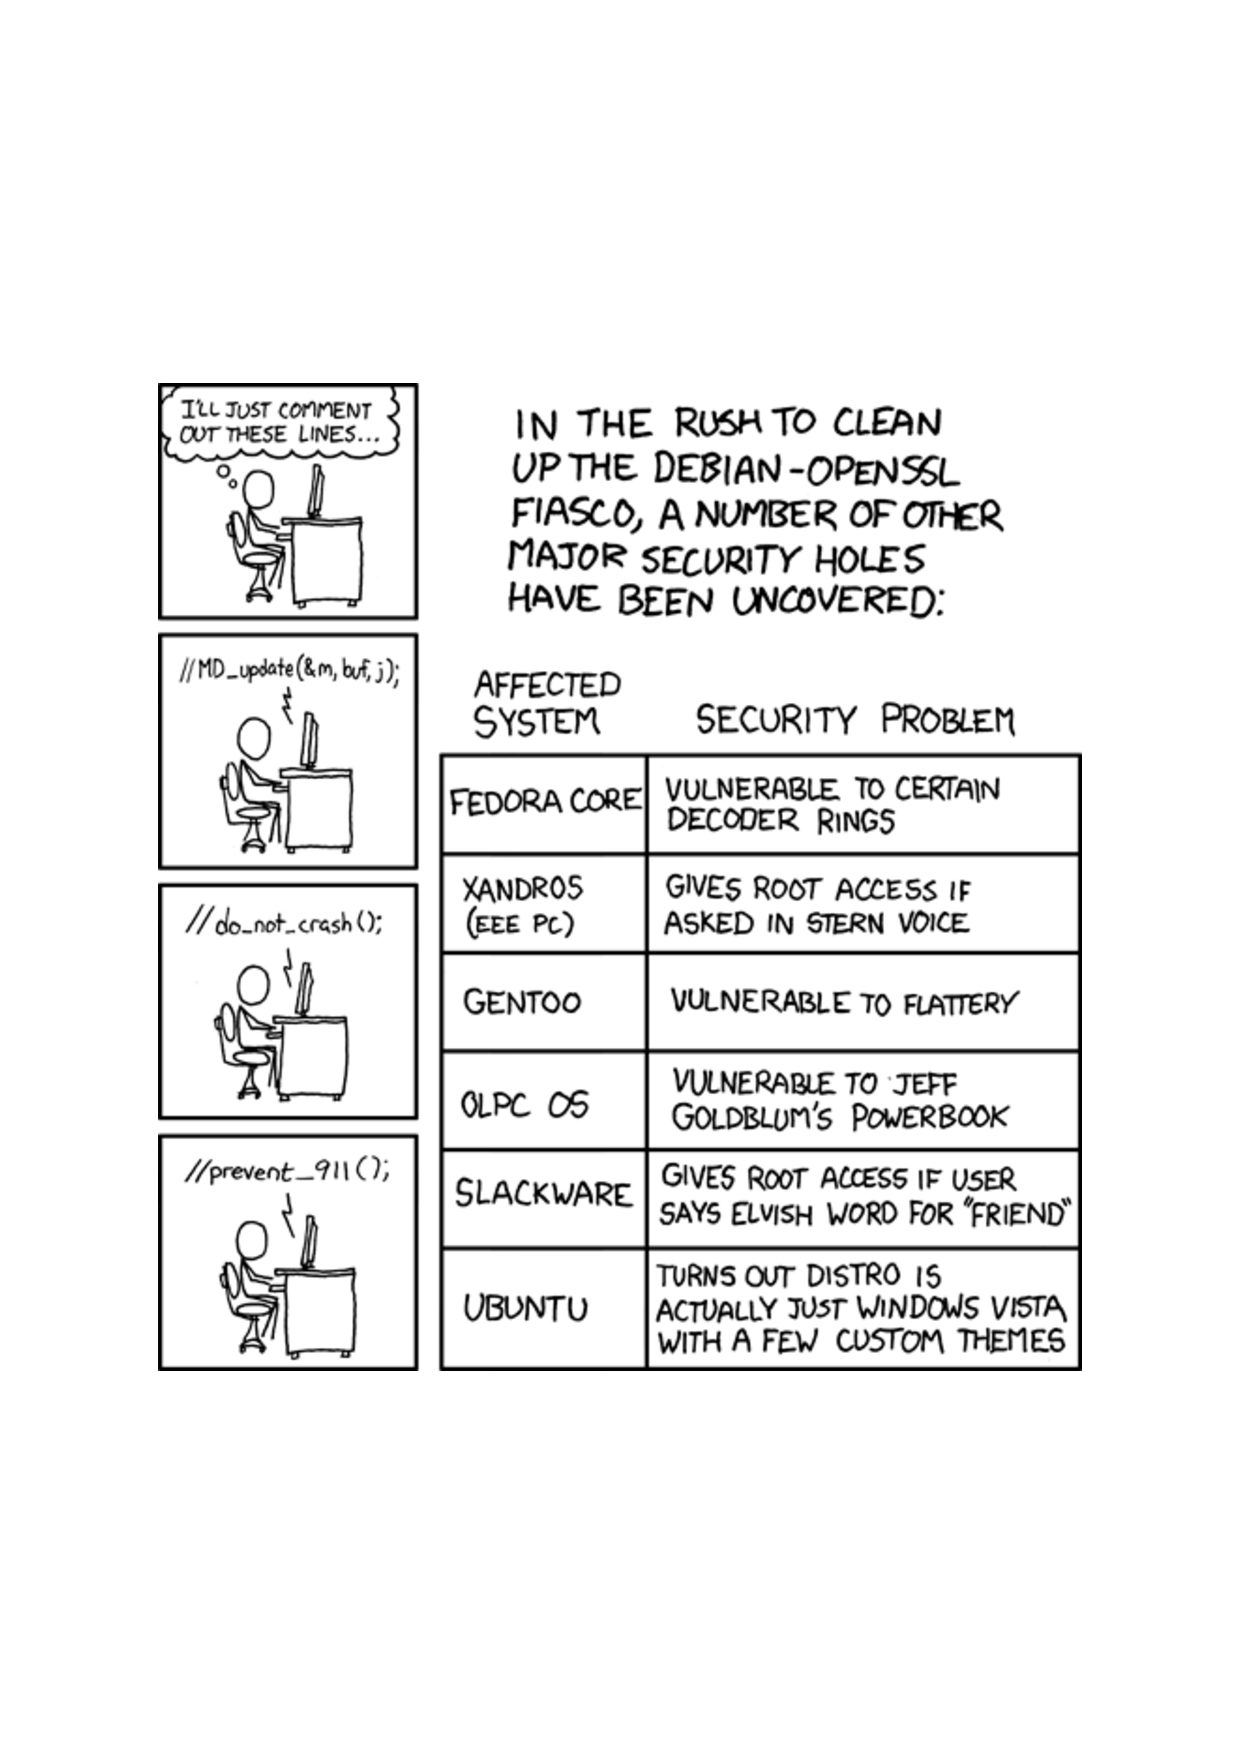
\includegraphics[width=60mm]{pic/holes} 
\end{center}
\end{figure}
\end{frame}
\section{Proof By Reduction}
\begin{frame}\frametitle{Reduction (Complexity)}
A \textbf{reduction} is a transformation of one problem $A$ into another problem $B$.
\newline

\textbf{Reduction} $A \le_m B$ \footnote{$m$ means the mapping reduction.} : $A$ is \textbf{reducible} to $B$ if solutions to $B$ exist and whenever given the solutions $A$ can be solved. \newline

Solving $A$ \textbf{cannot be harder} than solving $B$.
\begin{exampleblock}{Example}
\begin{itemize}
\item ``measure the area of a rectangle'' $\le_m$ ``measure the length and width of rectangle''
\item ``calculate $x^2$'' $\le_m$ ``calculate $x \times y$''
\end{itemize}
\end{exampleblock}
\end{frame}
\begin{frame}\frametitle{Proofs of Reduction}
\begin{figure}
\begin{center}
\input{tikz/reduction}
\end{center}
\end{figure}
\begin{itemize}
\item A \textsc{ppt} $\mathcal{A}$ can break $\Pi$ with probability $\varepsilon(n)$.
\item \textbf{Assumption}: Problem $\mathsf{X}$ is \emph{hard} to solve.
\item \textbf{Reduction}: Reduce $\mathcal{A}'$ to $\mathcal{A}$. $\mathcal{A'}$ solves $\mathsf{x}$ efficiently with probability $1/p(n)$, running $\mathcal{A}$ as a sub-routine. 
\item \textbf{Contradiction}: If $\varepsilon(n)$ is non-negligible, then $\mathcal{A'}$ solves $\mathsf{X}$ efficiently with non-negligible probability $\varepsilon(n)/p(n)$.
\end{itemize}
\end{frame}
\begin{frame}\frametitle{An Example of Proof By Reduction}
\begin{exampleblock}{If $F(s)$ is PRG, so is $G(s)=F(s)\oplus 1^{\abs{n}}$ ?}
\begin{itemize}
\item Problem A (Assumption): to distinguish $F(s)$ from $r$
\item Problem B (Break the scheme): to distinguish $G(s)$ from $r$
\end{itemize}
\textbf{Idea}: Reduce A to B. As $F(s)$ is distinguishable, so is $G(s)$.
\begin{figure}
\begin{center}
\begin{tikzpicture} %[scale=0.7, every node/.style={scale=0.7}]
\draw (0,0) rectangle (5,4);
\draw (3,0.5) rectangle (4.5,3);
\draw[-latex] (-3,3) -- (0,3) node [midway, above] {in $:= r$ or $F(s)$} node [midway, below] {};
\draw[-latex] (0,0.3) -- (-3,0.3) node [midway, above] {out};
\draw (1.8,3.5) node {$D'$ for $F$};
\draw (3.75,1.75) node {$D$ for $G$};
\draw[-latex] (0.5,2.5) -- (3,2.5) node [midway, above] {in $\oplus 1^{n}$ } node [midway, below] {};
\draw[-latex] (3,1) -- (0.3,1) node [midway, above] {out $= 0$ or $1$};
\end{tikzpicture}
\end{center}
\end{figure}
\end{exampleblock}
\end{frame}
\begin{frame}\frametitle{An Example of Proof By Reduction (Cont.)}
\begin{exampleblock}{If $F(s)$ is PRG, so is $G(s)=F(s)\oplus 1^{\abs{n}}$ ?}
\[ \Pr[D'(F(s))=1]=\Pr[D(G(s)=F(s)\oplus 1^n)=1] \]
\[ \Pr[D'(r)=1]=\Pr[D(r\oplus 1^n)=1]=\Pr[D(r)=1] \]
\[ \begin{split}
\mathsf{negl} &\ge \Pr[D'(F(s))=1] - \Pr[D'(r)=1] \\
              &= \Pr[D(G(s))=1] - \Pr[D(r)=1]
\end{split} \]
According to the definition of PRG, $G(s)$ is a PRG.
\end{exampleblock}
\end{frame}
\section{Constructing Secure Encryption Schemes}
\begin{frame}\frametitle{A Secure Fixed-Length Encryption Scheme}
\begin{columns}[t]
\begin{column}{4cm}
\begin{figure}
\begin{center}
\input{tikz/encryptionwithpg}
\end{center}
\end{figure}
\end{column}
\begin{column}{6cm}
\begin{construction}\label{con:fl}
\begin{itemize}
\item $|G(k)| = \ell(|k|)$, $m \in \{0,1\}^{\ell(n)}$.
\item $\mathsf{Gen}$: $k \in \{0,1\}^n$.
\item $\mathsf{Enc}$: $c := G(k)\oplus m$.
\item $\mathsf{Dec}$: $m := G(k)\oplus c$.
\end{itemize}
\end{construction}
\begin{theorem}\label{the:flt}
This fixed-length encryption scheme has indistinguishable encryptions in the presence of an eavesdropper.
\end{theorem}
\end{column}
\end{columns}
\end{frame}
\begin{frame}\frametitle{Proof of Indistinguishable Encryptions}
\textbf{Idea}: Use $\mathcal{A}$ to construct $D$ for $G$, so that $D$ distinguishes $G$ when $\mathcal{A}$ breaks $\tilde{\Pi}$. Since $D$ cannot distinguish $G$, so that $\mathcal{A}$ cannot break $\tilde{\Pi}$.
\begin{proof}
\begin{figure}
\begin{center}
\input{tikz/constructD}
\end{center}
\end{figure}
\[ \Pr[D(w)=1] = \Pr[\mathsf{PrivK}^{\mathsf{eav}}_{\mathcal{A},\tilde{\Pi}}(n)=1] \]
\end{proof}
\end{frame}
\begin{frame}\frametitle{Proof of Indistinguishable Encryptions (Cont.)}
\begin{proof}
To prove $ \varepsilon(n) \overset{\text{def}}{=} \Pr[\mathsf{PrivK}^{\mathsf{eav}}_{\mathcal{A},\Pi}(n)=1] - \frac{1}{2} $ is negligible.\\
(1) If $w$ is $r$ chosen \emph{u.a.r}, then $\tilde{\Pi}$ is OTP. \[\Pr[D(r)=1] = \Pr[\mathsf{PrivK}^{\mathsf{eav}}_{\mathcal{A},\tilde{\Pi}}(n)=1]=\frac{1}{2};\] \\
(2) If $w$ is $G(k)$, then $\tilde{\Pi} = \Pi$. 
\[ \Pr[D(G(k))=1] = \Pr[\mathsf{PrivK}^{\mathsf{eav}}_{\mathcal{A},\Pi}(n)=1] = \frac{1}{2} + \varepsilon(n). \]\\
Use Definition \ref{def:pg}: 
\[ \left|\Pr[D(r)=1] - \Pr[D(G(k))=1]\right| = \varepsilon(n) \le \mathsf{negl}(n).
\] 
\end{proof}
\end{frame}
\begin{frame}\frametitle{Handling Variable-Length Messages (homework)}
\begin{definition}\label{def:vlpg}
A \textbf{deterministic} polynomial-time algorithm $G$ is a \textbf{variable output-length pseudorandom generator} if
\begin{enumerate}
\item $G(s, 1^{\ell})$ outputs a string of length $\ell > 0$, where $s$ is a string.
\item $G(s, 1^{\ell})$ is a prefix of $G(s, 1^{\ell'})$, $\ell' > \ell$.\footnote{for technical reasons to prove security.}
\item $G_{\ell}(s) \overset{\text{def}}{=} G(s,1^{\ell(|s|)})$. Then $\forall \ell(\cdot)$, $G_{\ell}$ is a PRG with expansion factor $\ell$.
\end{enumerate}
\end{definition}
Both Construction \ref{con:fl} and Theorem \ref{the:flt} hold here.
\end{frame}
\begin{frame}\frametitle{Computational Security vs. Info.-theoretical Security}
\begin{center}
\begin{tabular}{|c|c|c|} \hline
                      & \textbf{Computational} & \textbf{Info.-theoretical} \\ \hline
\textbf{Adversary}    & \textsc{ppt} & no limited \\ 
                      & eavesdropping & eavesdropping\\ \hline 
\textbf{Definition}   & indistinguishable & indistinguishable \\ 
                      & $\frac{1}{2} + \mathsf{negl}$ & $\frac{1}{2}$ \\ \hline
\textbf{Assumption}   & pseudorandom & random   \\ \hline
\textbf{Key}	      & short random str. & long random str.\\ \hline
\textbf{Construction} & XOR pad & XOR pad \\ \hline 
\textbf{Prove}        & reduction & prob. theory  \\ \hline
\end{tabular}	
\end{center}
\end{frame}
\end{document}
